\chapter{Implementación de la aplicación}

\epigraph{\textit{''Talk is cheap. Show me the code''}}{--- Linus Torvalds}

Dentro del desarrollo de la aplicación, la parte que se puede considerar como la más importante es la parte de la implementación. Tomando en base todo el diseño, tanto a nivel conceptual, gráfico o de software, se ha implementado la aplicación, siendo esta uno de los dos objetivos del proyecto.

En este capítulo se explican los diferentes aspectos del proceso de desarrollo, tanto como se ha implementado la persistencia de datos, los escaneos que realiza la aplicación y todo tipo de consideraciones que se han tenido en cuenta durante la implementación y que merece la pena mencionar.

Este capítulo no pretende ser ni una descripción de cada elemento que forma parte del código, ni una documentación formal como puede ser la documentación de una API. Por razones de espacio y claridad, no se incluye todo el código desarrollado, tanto porque entorpecería las explicaciones de como se ha ido desarrollando y como se ha ido implementado la aplicación como porque haría este informe del proyecto excesivamente grande.

\section{Estructura del proyecto}
El código del proyecto se puede dividir en dos grandes bloques. Por una parte disponemos de los ficheros que contienen código en Kotlin y por otra parte los ficheros XML que definen, tanto layouts, elementos que se pueden dibujar o variables asociadas a las diferentes cadenas de caracteres (de ahora en adelante \textit{strings}) o a variables numéricas como colores o dimensiones.

El propio entorno de Android Studio permite diferencias ambos tipos de archivos, disponiendo del código en la carpeta \textit{java} (el nombre puede llevar a confusión, pero es el nombre por defecto en la creación de proyecto, aunque contenga únicamente código en Kotlin) y de los diferentes archivos XML en la carpeta \textit{res}. Esta última a su vez se divide en diferentes carpetas para organizar los archivos XML en función de su utilidad.

\begin{figure}[H]
	\centering
	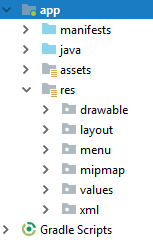
\includegraphics{basic-android-studio-structure}
	\caption{Estructura básica de archivos del proyecto}
	\label{fig:basic-android-studio-structure}
\end{figure}

Otras carpetas importantes son las carpetas de \textit{manifests} y la carpeta de \textit{assets}. En la primera es donde se guardan los diferentes \textit{Manifest} de la aplicación. Un Manifest\footnote{\url{https://developer.android.com/guide/topics/manifest/manifest-intro}} en Android es un fichero XML donde se definen una serie de variables importantes a nivel global con respecto a la aplicación. Entre otras funciones, es donde se define el nombre de la aplicación, su icono y sus diferentes componentes, que pueden ser Activities, Services, BroadcastReceivers o ContentProviders.

Por otra parte mencionar la existencia de diferentes scripts de Gradle, que es el sistema de automatización de construcción de aplicaciones más usado en Android para compilar el código y generar la aplicación ejecutable, entre otras cosas.

\subsection{Estructura de paquetes de código}

Dentro de la carpeta \textit{java}, debido a la gran cantidad de ficheros de código Kotlin, existe una estructura de paquetes que divide los ficheros de código en diferentes categorías. Cada uno de los ficheros de código existentes implementa una única clase, interfaz o tipo enumerado. Esto es así para mantener cada elemento claramente visible y al mismo nivel y a su vez evitar archivos excesivamente grandes que compliquen entender el código. La estructura de paquetes se muestra en la Figura \ref{fig:android-studio-package-structure}.

\begin{figure}[H]
	\centering
	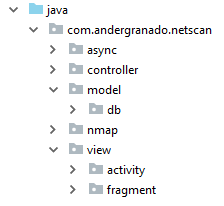
\includegraphics{android-studio-package-structure}
	\caption{Estructura de paquetes de código del proyecto}
	\label{fig:android-studio-package-structure}
\end{figure}

En los paquetes \textit{model}, \textit{controller} y \textit{view} se implementan las diferentes partes de las que está formada una aplicación que sigue el patrón MVC (Model View Controller). Es un patrón largamente usado a la hora de diseñar aplicaciones con interfaz gráfica, que consiste básicamente en dividir los datos (Model), las diferentes vistas de la aplicación (View) y la parte que actúa como puente entre los datos y las vistas (Controller) en entidades separadas. Esto permite que el codigo generado sea escalable, legible y elimine dependencias innecesarias. 

En el caso de Android, las diferentes vistas se implementan en diversas Acitivities y Fragments. El modelo es básicamente una serie de clases (algunas de ellas Data Classes de Kotlin) que definen los diferentes datos que existen, tanto para la aplicación como datos concretos que son persistentes en la aplicación (separados en el paquete \textit{db}) y los controladores están implementados usando RecyclerViews de Android, cuyo funcionamiento se explicará más adelante.

Por último, mencionar los paquetes \textit{async} y \textit{nmap}. El paquete \textit{async} contiene toda aquella funcionalidad que se ejecuta de manera paralela o asíncrona, como diferentes AsyncTasks o clases que se basan en la ejecución de Threads o hilos. El paquete \textit{nmap} contiene todo el código necesario para implementar Nmap en la aplicación, tanto para instalarlo, ejecutarlo como para interpretar los datos que genera. Todo el código que hace uso de Nmap se encuentra en este paquete, dejando el resto de la aplicación completamente aislada de las particularidades de Nmap

\section{Integración de Nmap}

Integrar soluciones de terceros en una aplicación o un sistema que está en desarrollo puede ser desde algo simple, más bien mecánico, a todo un quebradero de cabeza, en función del tipo de software o funcionalidad que queramos añadir desde fuera.

En concreto, a la hora de integrar Nmap en la aplicación hay que tener en cuenta una serie de factores. Integrar Nmap en una aplicación difiere completamente de integrar, por ejemplo, una librería con una API definida. Integrar una librería en una aplicación consiste simplemente en una serie de pasos para configurar esa librería que, una vez realizados, nos permiten mediante una interactuar mediante una API con esa librería y aprovechar toda la funcionalidad que nos provee. 

En cambio, con Nmap es radicalmente diferente. Debido a que Nmap no es una librería, sino un software complejo que nos permite analizar redes de ordenadores, no podemos integrarlo como si de una librería se tratase. Por lo tanto, debemos buscar otros métodos diferentes para integrarlo.

Nmap es una solución de código libre que lleva siendo desarrollada por la comunidad que ha generado alrededor durante más de 10 años. Cabría pensar que una posibilidad para integrar la funcionalidad de Nmap en la aplicación es obtener su código fuente (que al ser software libre es público y está disponible para su uso) e integrarlo directamente en el proyecto.

El principal problema de esta posibilidad es que Nmap es un software muy complejo. El núcleo de Nmap está desarrollado en C, pero también diversas partes están desarrolladas en lenguaje es como Lua, C++ o Python, como se puede observar en la FIGURA de su repositorio\footnote{\url{https://github.com/nmap/nmap}}. Esto impide que podamos introducir todo ese código en lenguajes no soportados por Android en el proyecto, haciendo que Nmap no se pueda integrar directamente a nivel de código.

\begin{figure}[H]
	\centering
	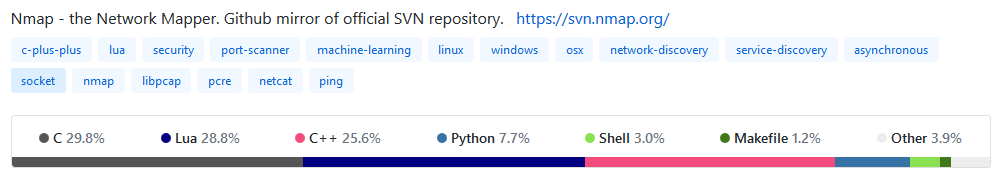
\includegraphics[width=1.0\textwidth]{nmap-repo-languages}
	\caption{Distribución de lenguajes en el repositorio de Nmap}
	\label{fig:nmap-repo-languages}
\end{figure}

Es cierto que se puede, mediante el uso del NDK de Android, introducir código tanto en C como en C++ en nuestra aplicación. Pero el funcionamiento de Nmap es tan complejo que intentar integrar solamente esa parte del código y esperar que funcione eliminando el resto de módulos sería una tarea tan titánica como inútil.

Por ello la última opción, y la única realmente viable, para integrar Nmap en nuestra aplicación es interactuar directamente con archivos binarios de Nmap. Es decir, incluir la aplicación compilada dentro del proyecto, ejecutarla mediante código y obtener e interpretar la información que devuelva.

\subsection{Instalación}

Esto a la vez genera una serie de cuestiones. Si queremos introducir un binario dentro de nuestra aplicación y controlar su ejecución en un dispositivo lo primero que tenemos que tener en cuenta es que la arquitectura para la que ha sido compilada el binario coincida con la arquitectura del dispositivo.

Nmap  es una aplicación que se puede ejecutar tanto en sistemas Windows y OS X como en sistemas basados en Linux. Aunque android es un sistema Linux, Android no se suele ejecutar en las plataformas en las que se suele ejecutar normalmente Linux, que son x86 y x64, arquitecturas Intel. La mayor parte de dispositivos Android son dispositivos con procesadores ARM BUSCAR REFERENCIA,por lo tanto no podemos  ejecutar una versión estándar de Nma para Linux.

Para solucionar esto se puede optar por dos opciones. La primera sería compilar Nmap para arquitecturas especialmente para Android en ARM. Compilar un proyecto de la envergadura de Nmap es una tarea engorrosa y difícil de realizar. La segunda sería buscar binarios ya compilados especialmente para Android. Por suerte existen binarios de Nmap para dispositivos Android.

La propia web de Nmap\footnote{\url{https://secwiki.org/w/Nmap/Android}} nos ofrece binarios de Nmap específicos para Android, la desventaja es que no se trata de binarios oficiales, aunque avalados por Nmap, sino de binarios generados por un usuario concreto\footnote{\url{https://github.com/kost/nmap-android}}. Otra desventaja de estos binarios es que no están completamente actualizados. La versión más reciente de los binarios de Nmap para Android es la 7.31 (25 de octubre de 2016), unas versiones más atrasada desde la última, la 7.70\footnote{\url{http://seclists.org/nmap-announce/2018/0}} (20 de marzo de 2018) que a día de hoy es la última versión de Nmap.

Aunque la última versión disponible de Nmap para Android no está tan actualizada como la última versión de Nmap, hay que tener en cuenta que Nmap es un software con un desarrollo avanzado y que, aunque vaya añadiendo funcionalidad, lleva durante años siendo un software robusto y estable. Por esto utilizar Nmap para Android no debería ser un gran problema.

Nmap para Android viene compilado o para una serie de arquitecturas concretas, como se puede observar en la FIGURA. Aunque tenemos un rango amplio de arquitecturas para elegir, debemos tener en cuenta que nuestro público objetivo es un público general. La mayor parte de móviles Android utilizan procesadores ARM. Aun así, y para garantizar la compatibilidad con todos los dispositivos, se han integrado binarios de Nmap para Android para arquitecturas ARM. x86 y MIPS, con sus equivalentes de 64 bits. Con esto cubriremos todos los dispositivos móviles posibles.

\begin{figure}[H]
	\centering
	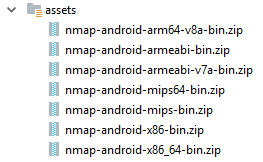
\includegraphics{project-assets}
	\caption{Los diferentes binarios para cada arquitectura usados en la aplicación}
	\label{fig:project-assets}
\end{figure}

La forma de introducir estos binarios en el dispositivo es sencilla y está completamente automatizada. por una parte se almacena cada uno de los diferentes binarios en diferentes ficheros comprimidos en formato ZIP. Cada uno de estos ficheros ZIP se encuentra metido en la carpeta \textit{assets} del proyecto, como se muestra en la Figura \ref{fig:project-assets}. Esta carpeta sirve para guardar todo tipo de recursos que queramos cargar en nuestra aplicación. Recursos como pueden ser ser archivos de texto, imágenes, archivos de audio, y un largo etcétera. Aunque en principio no esté diseñada para guardar binarios y programas completos, en nuestro caso servirá para guardar los ficheros de Nmap y después poder desplegarlos en el dispositivo.

Desplegarlos en el dispositivo es relativamente sencillo. Para ello solo debemos tener en cuenta la arquitectura el dispositivo en el que se está ejecutando la aplicación y descomprimir el archivo con los binarios correspondientes.

La localización donde guardemos los binarios de Nmap es fundamental, ya que según donde se guarden tendremos permiso para ejecutarlos o no. En este caso se guardan en lo que denominamos Internal Storage\footnote{\url{https://developer.android.com/training/data-storage/files}} de Android. Dentro de la estructura de archivos de Android existe una carpeta llamada \textit{data}, que a su vez tiene otra carpeta del mismo nombre. Dentro de esa última carpeta existe una carpeta por cada aplicación instalada en el sistema. Cada una contiene una aplicación y sus archivos asociados. Esta carpeta sólo es accesible para la propia aplicación, que tiene permisos de lectura, escritura y ejecución dentro de ella, lo que la convierte en el lugar idóneo para depositar los binarios.

Toda este volcado de binarios de Nmap para el dispositivo se gestiona desde una única clase en la aplicación llamada \mintinline{java}{NmapInstaller}. Esa clase, que implementa el patrón Singleton mediante el uso de la palabra clave \mintinline{java}{object} de Kotlin, contiene todo el código necesario para volcar los binarios de Nmap en el dispositivo.

\begin{listing}[H]
	\inputminted[
	tabsize=4,
	frame=single,
	framesep=2mm,
	baselinestretch=1.0,
	fontsize=\scriptsize,
	linenos,
	breaklines
	]{kotlin}{code/install.kt}
	\caption{Función que instala Nmap en el dispositivo}

	\label{code:install}
\end{listing}

Como se puede observar en el código, dentro de la función \mintinline{java}{install()} se realiza ese volcado pudiendo tener opciones para reescribir los archivos en caso de que se quiere escribir. Estos archivos se cargan a través del Asset Manager y mediante las clases de Java para interactuar con ficheros comprimidos se extraen en los ficheros internos de la aplicación.

A su vez también se actualiza la base de datos de script NSE de Nmap, en caso de que se quiera después ejecutar alguno de esos script. 

\subsection{Ejecución}

Una vez tenemos disponibles todos los binarios de Nmap y archivos necesarios para ejecutar Nmap introducidos e instalados en el dispositivo, el siguiente paso necesario es implementar la funcionalidad que nos permita ejecutarlos.

Todo el código que permite ejecutar en el mapa se encuentra en otra clase llamada \mintinline{java}{NmapRunner}. Esta clase tiene diversos métodos que nos permiten interactuar con los binarios y en última instancia ejecutar escaneos.

Lo que tenemos que hacer para ejecutar un escaneo es ejecutar el binario de Nmap con los parámetros correspondientes. Para ejecutar en el mar basta simplemente con lanzar un proceso que llame a la ejecución del binario. La forma de ejecutar un binario es muy sencilla, y consiste en crear un proceso para una shell de Linux y en el llamar al ejecutable de Nmap. Para poder interactuar con ese proceso necesitamos configurar la entrada y la salida de ese proceso para poder enviarle información y recibirla. Eso se realizan la función \mintinline{java}{startProcess()}, que se muestra a continuación.

\begin{listing}[H]
	\inputminted[
	tabsize=4,
	frame=single,
	framesep=2mm,
	baselinestretch=1.0,
	fontsize=\scriptsize,
	linenos,
	breaklines
	]{kotlin}{code/startProcess.kt}
	\caption{Función para arrancar el proceso con la shell que ejecutará Nmap}
	
	\label{code:startProcess}
\end{listing}

Después de esto debemos construir un comando de Nmap. Este comando es básicamente lo que haríamos si estuviéramos ejecutando Nmap en la terminal de nuestro ordenador. En nuestro caso solo queremos realizar una serie de escaneos concretos a nodos puntuales, por lo tanto construir este comando es tan sencillo como concatenar unos pocos strings. La función que realiza esto se muestra a continuación.

\begin{listing}[H]
	\inputminted[
	tabsize=4,
	frame=single,
	framesep=2mm,
	baselinestretch=1.0,
	fontsize=\scriptsize,
	linenos,
	breaklines
	]{kotlin}{code/commandBuilder.kt}
	\caption{Función que crea el comando a ejecutar de Nmap}
	
	\label{code:commandBuilder}
\end{listing}

Una vez realizado esto queda pasar ese comando al proceso y ejecutar Nmap. A partir de aquí podríamos obtener la información del escaneo de dos maneras. La primera sería leer la salida que nos da el proceso en texto plano y extraer la información de. La segunda, mejor alternativa, consiste en ejecutar Nmap de tal manera que la información del escaneo se guarde en un fichero XML.

Las ventajas de utilizar un fichero XML para cobrar esa información son obvias. En un fichero XML dispondremos de la información estructurada que podremos leer utilizando la librería para trabajar con archivos XML que provee el SDK de Android. Por lo tanto, y como se ha podido observar, se añade el parámetro \mintinline{java}{-oX} cuándo se crea el comando a ejecutar, qué es el que indica que la salida se almacene en un fichero XML.

Una vez realizado el escaneo y habiéndose generado ese fichero XML, solo queda obtener la información de ese fichero y deshacernos de todos los recursos ya innecesarios, como el propio fichero XML una vez leído, o el propio proceso de la shell, que consume recursos no necesarios.

\begin{listing}[H]
	\inputminted[
	tabsize=4,
	frame=single,
	framesep=2mm,
	baselinestretch=1.0,
	fontsize=\scriptsize,
	linenos,
	breaklines
	]{kotlin}{code/runScan.kt}
	\caption{Función con todo el proceso de ejecución de un escaneo en Nmap}
	
	\label{code:runScan}
\end{listing}

\subsection{Leer datos}

La tercera y última parte del proceso para integrar Nmap es leer los datos que han sido generados. Como se ha mencionado dichos datos se encuentran en un fichero XML. Por lo tanto, necesitaremos una clase qué obtenga la informacion de dicho fichero. A este tipo de clases se le suele denominar \textit{parser} y básicamente van leyendo las diferentes etiquetas de los ficheros XML y obteniendo su información. A continuación se muestra ciertas partes del código para hacerse la idea de cómo es leer de manera jerarquizada y estructura de un fichero XML. No se muestra toda la implementación, ya que el tamaño de la implementación de un parser de XML es directamente proporcional al tamaño de la jerarquía de los elementos que contiene.

\begin{listing}[H]
	\inputminted[
	tabsize=4,
	frame=single,
	framesep=2mm,
	baselinestretch=1.0,
	fontsize=\tiny,
	linenos,
	breaklines
	]{kotlin}{code/nmapParser.kt}
	\caption{Extracto de la implementación de un parser de un XML de Nmap}
	
	\label{code:nmapParser}
\end{listing}

Almacenar la información en XML la almacena jerarquizada en cierta manera la manera en la que Nmap guarda información estructurada en un fichero XML es como la que se muestra en el Código \ref{code:regular-scan}:

\begin{listing}[H]
	\inputminted[
	tabsize=4,
	frame=single,
	framesep=2mm,
	baselinestretch=1.0,
	fontsize=\tiny,
	linenos,
	breaklines
	]{xml}{code/regular-scan.xml}
	\caption{Fichero XML con la información de un escaneo estándar de Nmap}
	
	\label{code:regular-scan}
\end{listing}

Sin entrar en detalles sobre el funcionamiento cada una etiqueta se puede observar que se genera una etiqueta \textit{host} por cada uno de los nodos encontrados en el escaneo. Un solo escaneo puede servir tanto para único host como para un rango completo de redes CIDR, por lo que habrá tantas etiquetas host como nodos se hayan detectado.

Dentro de la información generada para cada host, aunque depende del tipo de escaneo realizado, se pueden observar etiquetas que aparecerán para la gran mayoría de casos. Por ejemplo \textit{status}, que nos indica el estado del host, \textit{address}, que nos indica la dirección IP del host, \textit{hostname},que es el nombre que recibe dicho host, o la etiqueta \textit{ports}, qué contiene una lista de todos los puertos abiertos o filtrados que se han encontrado para cada nodo, con información sobre configuraciones, métodos usados para escanearlos o nombres de dichos puertos.

Por último una vez leído ese fichero a medida que se va leyendo ese fichero se va guardando la información en diferentes clases, creadas específicamente para guardar los datos obtenidos de Nmap antes de ser procesados. Dichas clases se encuentran dentro del paquete \textit{model}. En concreto, todas las clases que se usan para datos obtenidos directamente de Nmap llevan el prefijo \mintinline{java}{Nmap}, para diferenciarlas de clases del modelo relacionadas con la estructura de la información en la base de datos. En los Códigos \ref{code:nmapScan}, \ref{code:nmapHost} y \ref{code:nmapPort} se muestran unos ejemplos.

\begin{listing}[H]
	\inputminted[
	tabsize=4,
	frame=single,
	framesep=2mm,
	baselinestretch=1.0,
	fontsize=\scriptsize,
	linenos,
	breaklines
	]{kotlin}{code/nmapScan.kt}
	\caption{Data Classes para la información de un scan en Nmap}
	
	\label{code:nmapScan}
\end{listing}

\begin{listing}[H]
	\inputminted[
	tabsize=4,
	frame=single,
	framesep=2mm,
	baselinestretch=1.2,
	fontsize=\scriptsize,
	linenos,
	breaklines
	]{kotlin}{code/nmapHost.kt}
	\caption{Data Classes para la información de un host en Nmap}
	
	\label{code:nmapHost}
\end{listing}

\begin{listing}[H]
	\inputminted[
	tabsize=4,
	frame=single,
	framesep=2mm,
	baselinestretch=1.0,
	fontsize=\scriptsize,
	linenos,
	breaklines
	]{kotlin}{code/nmapPort.kt}
	\caption{Data Classes para la información de un puerto en Nmap}
	
	\label{code:nmapPort}
\end{listing}

\section{Persistencia de datos}

\section{Obtención de información de medios externos}

\section{Hilos, Tareas y paralelización}

\section{Interfaz gráfica}


